\documentclass[letterpaper,12pt]{article}
\usepackage{cite}
\usepackage{float}
\usepackage{listings}
\usepackage{graphicx}
\usepackage{tikz}
\usepackage{pgfplots}
\graphicspath{ {images/} }

\title{Line detection via the Hough transform}
\date{December 23, 2015}
\author{Ryan Zoeller}

\begin{document}
\bibliographystyle{unsrt}
\maketitle

\begin{abstract}
The generalized Hough transform provides a convenient technique for detecting features in an image --
in the classical case, lines.
A thresholded edge matrix is generated for the image (using any one of a number of edge detection
operators, e.g. the Sobel operator); this matrix is then used in a voting process carried
out in a parameter space. In the classical Hough transform this parameter space is the polar
normal form of a line, which is especially useful as it allows for the constrained
search space $\theta \in (-\pi,\pi]$ as well as for representation of vertical lines.
This paper presents a multithreaded implementation of the classical Hough transform.
\end{abstract}

\newpage

\section{Introduction}
In the generalized (as well as classical) Hough transform, an edge matrix is generated
for the input image through two-dimensional image convolution. In practice, a variety of image
kernels are used for this convolution, including the Sobel, Scharr and Prewitt operators.
The edge matrix is then thresholded, producing a set of non-zero coordinate pairs.
These coordinate pairs are the input to the accumulation procedure used to detect prominent
features -- which, in the case of the classical Hough transform, are lines.
\\
In the classical Hough transform, the parameter space used for vote accumulation represents
the polar normal form of a line, which is given by $\rho=x*\cos{\theta}+y*\sin{\theta}$.
It has several advantages over the traditional point-slope equations, namely that the search
space is bounded. In the traditional point-slope form, the slope may approach both positive
and negative infinity; the representation of vertical lines requires this. Instead, the
polar normal form allows the entire range of theta to be swept using some small increment.

\section{Related Work}
The Hough transform was first described by Paul Hough in a 1962 patent\cite{paulhough1962},
although the description was purely geometric and no algebraic formulation was given.
The algorithmic foundation for this implementation is the 1972 work of Richard Duda
and Peter Hart\cite{dudahart1972}. A popular implementation of the Hough transform is
given by the OpenCV source.
\\
An alternative feature detection method to the generalized Hough transform is the Radon transform,
an integral transform introduced by Johann Radon in 1917. It has been shown that the Hough transform
is equivalent to the Radon transform in the continuous case\cite{radonhough}.

\section{Challenges}
\label{sec:chal}
While using a polar normal representation as the vote accumulation space is
conceptually better than the using point-slope form, the implementation of
the Hough transform in general presents some challenges. Most significant is
the high computational cost of the algorithm, which is in many ways hidden by
the algorithm's asymptotic complexity, as well as the direct correlation between
numerical accuracy and the constant factor abstracted by this complexity in
big $\mathcal{O}$ notation.

\subsection{Asymptotic Complexity}
The cost of computing the edge matrix using image convolution is $\mathcal{O}(mn)$ for
an image of dimensions $m$ by $n$. For a square image, this is equivalent to $\mathcal{O}(n^{2})$.
The cost of convolving each element is linear with the number of entries in the kernel, however
this cost is dominated by the cost of convolution as the kernel is required to be smaller than
the input image. Finding the entries of the edge matrix which satisfy some threshold is also linear with
the number of elements in the input image (i.e. $\mathcal{O}(mn)$ in the general case of an $m$
by $n$ image).
\\
The majority of the computational cost of the Hough transform instead stems from the
$\mathcal{O}(n)$ search of the parameter space, which is simply linear with the number of
thresholded points. While this is asymptotically dominated by the image convolution cost,
in practice the increment used to search the range of theta (or any other parameterized value)
is small, leading to a high constant factor. In the presented implementation, 1000 values of
theta are sampled for each candidate point.

\subsection{Numerical Precision}
The accuracy of the computed feature (in the classical case, a line) is proportional to the
precision of the discretized parameter space. Unfortunately, the computational cost is also
directly proportional to this precision. As a result, it is extremely important to determine
the required precision before generating the accumulation matrix, to avoid a result outside
the required tolerance or a result which is excessively expensive to compute.
\\
A further challenge the generalized Hough transform faces is the limit of floating point
precision. As the precision of the discretized parameter space increases, the impact of
numerical error also increases. Since the accumulation matrix is used to directly calculate
the most prominent features, these numerical errors can distort the actual results. At some
precision (before the machine epsilon is reached), the result is no longer meaningful, as
numerical error will contribute to neighboring vote buckets instead of the true vote bucket.
The result of this is either that the actual value will not statistically stand out
(i.e. neighboring buckets will have approximately the same value) or that a neighboring value
will succeed the actual value. One potential solution to this is to 'smear' the votes over a
region, i.e. to spread the vote across multiple buckets in a weighted fashion. This feature
is not present in the presented implementation however, due to performance and weighting concerns.

\section{Implementation}
The Classical Hough Transform could be implemented as shown in Listing \ref{lst:houghalg}.

\begin{lstlisting}[frame=tb,mathescape,caption={Hough transform algorithm},label={lst:houghalg}]
E := edge matrix calculated via image convolution
acc := dim. (1 + 2 * $\rho_{max}$) by (number of $\theta$ values)
thresholded := {}
for each pixel p $\in$ E:
    if (p.value $\geq$ threshold):
        thresholded := thresholded $\cup$ {(p.$x$, p.$y$)}
for each ($x$, $y$) $\in$ thresholded:
    for each $\theta \in (-\pi, \pi]$:
        $\rho$ := $x * \cos{\theta} + y * \sin{\theta}$
        $\hat{\rho}$ := round $\rho$ to nearest value in acc
        acc[$\hat{\rho}$, $\theta$] := acc[$\hat{\rho}$, $\theta$] + 1
return coordinates of local maxima of acc
\end{lstlisting}

The presented implementation deviates from Listing \ref{lst:houghalg} in order to attack
the challenges discuseed in Section \ref{sec:chal} in two ways. First, by subdividing the
interval of theta in the parameter space, multiple cores are able to share the load. In this way,
the lower bound for the wall time of the vote accumulation process is reduced to $1/n$, where $n$
is the number of threads sharing the work. Additionally, by ordering the loops such that modifying
theta is the outer loop and calculating rho for each thresholded point is the inner loop, the
calculations of $\sin{\theta}$ and $\cos{\theta}$ are reused. The calculation of these two
trigonometric functions for each theta is by far the most expensive part of the loop\cite{agnerfog2014}
-- unfortunately, modern compilers do not appear to be able to interchange the loops and hoist the
calculations out automatically.
\\
Despite the largely component-wise computations required by the Hough transform, an existing
linear algebra package (Armadillo) was chosen to represent the parameter space for several
reasons. The package provides compile-time switching of bounds checking via a macro, which enables
more thorough debugging as well as high performance in the final executable. Additionally, the
package provides convenient definitions for common functions such as the component-wise square root
and finding the coordinates of all entries larger than some threshold.

\section{Results}
The correctness of the presented implementation is demonstrated in Figures \ref{fig:unobscuredinput},
\ref{fig:obscuredinput}, \ref{fig:unobscuredoutput}, and \ref{fig:obscuredoutput}, in which
the correct feature is detected in both the unobscured and obscured cases.

\begin{figure}[H]
    \center{\frame{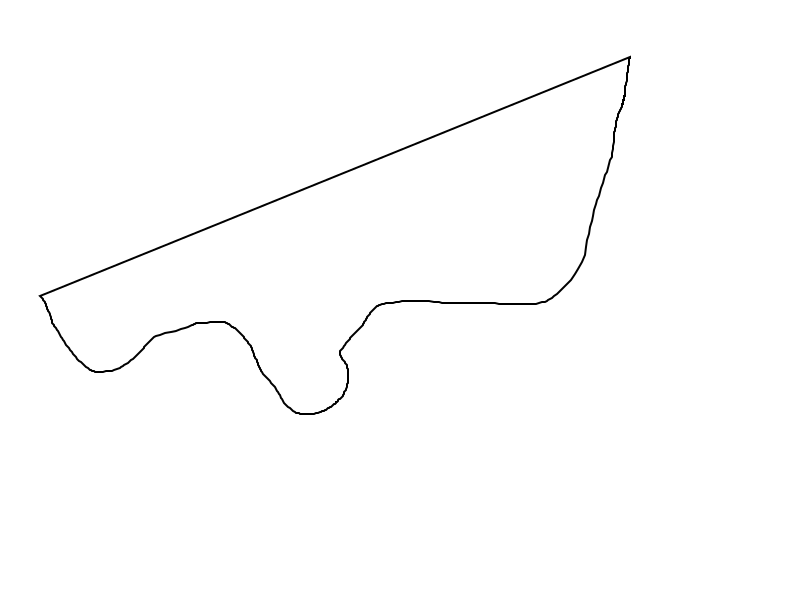
\includegraphics[width=8cm]{inputA.png}}}
    \caption{Unobscured input image}
    \label{fig:unobscuredinput}
\end{figure}

\begin{figure}[H]
    \center{\frame{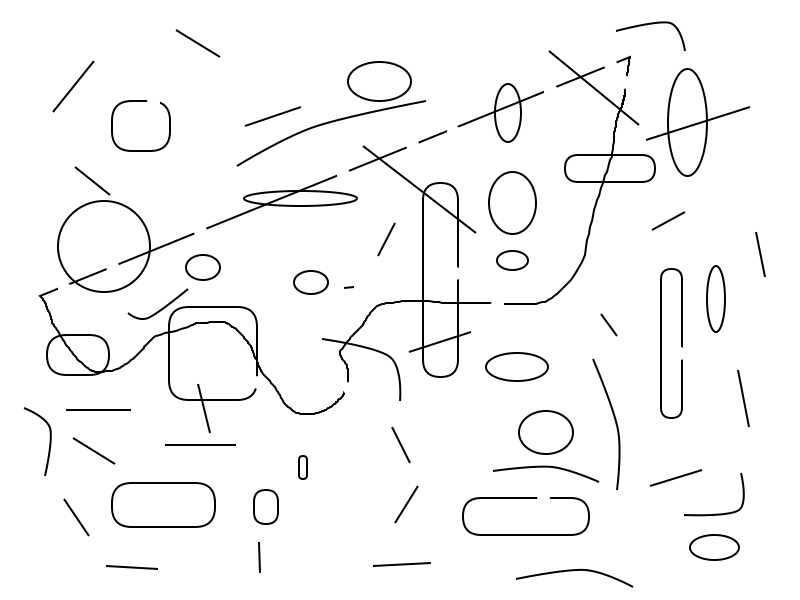
\includegraphics[width=8cm]{inputB.png}}}
    \caption{Obscured version of Figure \ref{fig:unobscuredinput}}
    \label{fig:obscuredinput}
\end{figure}

\begin{figure}[H]
    \center{\frame{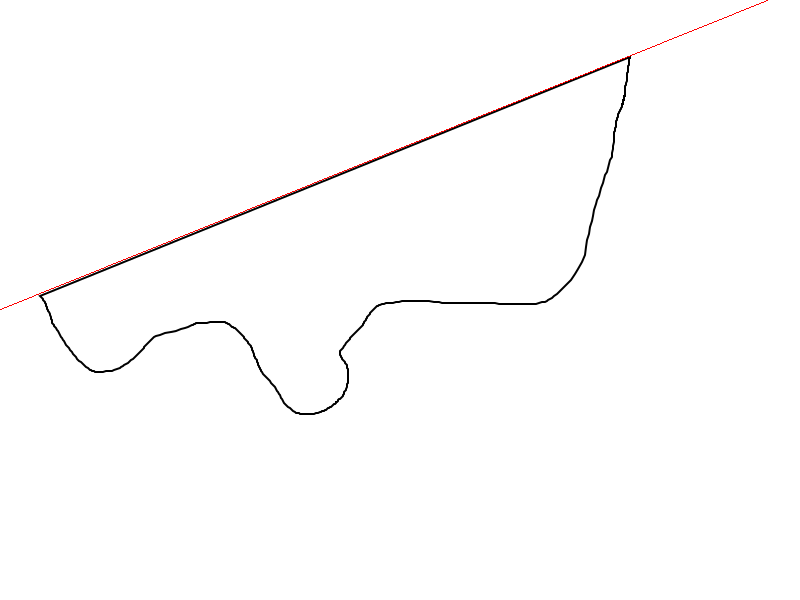
\includegraphics[width=8cm]{outputA.png}}}
    \caption{Output of Hough transform on Figure \ref{fig:unobscuredinput}}
    \label{fig:unobscuredoutput}
\end{figure}

\begin{figure}[H]
    \center{\frame{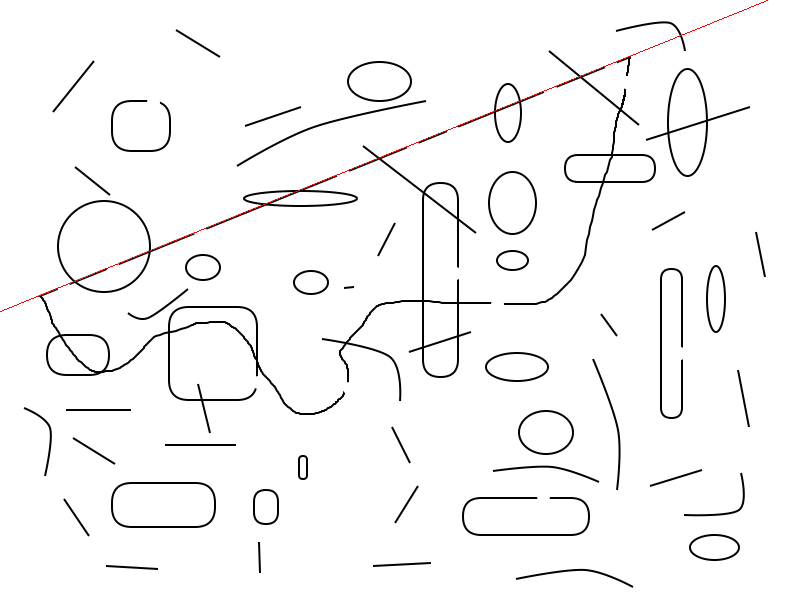
\includegraphics[width=8cm]{outputB.png}}}
    \caption{Output of Hough transform on Figure \ref{fig:obscuredinput}}
    \label{fig:obscuredoutput}
\end{figure}
The multithreaded implementation of the parameter space search provides a dramatic performance increase,
as seen in Figure \ref{fig:graph}, which reflects the execution time of the Hough transform of Figure \ref{fig:unobscuredinput},
averaged over ten trials (not including removed outliers). The sparsity of edges in Figure \ref{fig:unobscuredinput}
is responsible for the relatively high non-parallelized constant factor (i.e. where the execution time levels off) in
comparison to the execution time of the parallelized inner loop; this factor will remain approximately constant as the number
of edge pixels (and thus overall execution time) increases.

\begin{figure}[H]
    \center{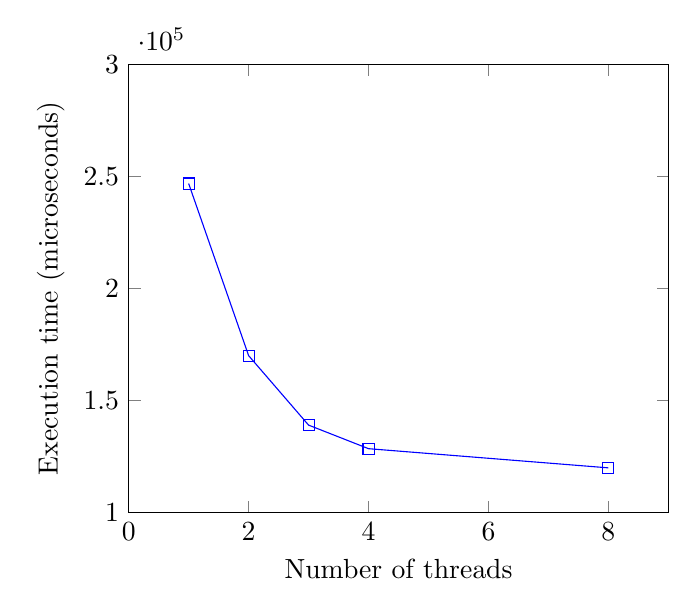
\begin{tikzpicture}
        \begin{axis} [xlabel={Number of threads},
                        ylabel={Execution time (microseconds)},
                        xmin=0,
                        xmax=9,
                        ymin=100000,
                        ymax=300000]
            \addplot[color=blue,mark=square] coordinates {(1,246742) (2,169985) (3,138997) (4,128476) (8,119922)};
        \end{axis}
    \end{tikzpicture}}
    \caption{Diminishing returns of a multithreaded approach}
    \label{fig:graph}
\end{figure}

The computations in Figure \ref{fig:graph} were performed on an Intel Core i7 4700MQ using the CFQ scheduler.
While the hardware implements eight threads, there are only four physical cores. As a result, the potential
performance benefits associated with the eight-thread parallelization are likely understated.

\section{Conclusion}
\subsection{Conclusions}
This paper presents a multithreaded implementation of the classical Hough transform and a discussion
of the challenges faced in computing the transform.
Parallelizing the Hough transform can be done na\"{\i}vely through clever partitioning of the parameter space.
In the non-sparse case, the performance benefits of this can be significant; for sparse edge matrices any performance
benefits are likely dominated by the cost of thread creation.
\\
While parallelization of the image convolution is possible (as with the partitioning of the parameter space,
this can be done na\"{\i}vely), the convolution process did not contribute significantly to the overall
runtime of the transform in images. If a more complex image kernel is used, it may be desirable to distribute the
computation, however the overhead of thread creation will likely dominate any perfomance benefits achieved for
most image sizes.

\subsection{Future Work}
Future work will likely include further restructuring of the parameter space iteration to support vectorization.
Additional research could enable the program to self-manage the thread creation based on the sparsity of the edge
matrix and the granularity of the search space. The representation of the accumulation matrix could potentially
be switched to a sparse implementation, as a large percentage of the accumulation matrix remains zero throughout
the computation (this can be illustrated by running the presented implementation in verbose mode and examining
the resulting heatmap).

\newpage
\bibliography{HoughWriteup}
\end{document}
